\newpage
\section{La Loi Normale (ou Gaussienne)}

\subsection{Introduction et Fonction de Densité (PDF)}

\begin{definitionbox}[Loi Normale]
Une variable aléatoire continue $X$ suit une \textbf{loi normale} (ou loi de Gauss) de paramètres $\mu$ (l'espérance) et $\sigma^2$ (la variance), notée $X \sim \mathcal{N}(\mu, \sigma^2)$, si sa fonction de densité de probabilité (PDF) est donnée par :
$$ f(x; \mu, \sigma) = \frac{1}{\sigma \sqrt{2\pi}} e^{ -\frac{1}{2} \left( \frac{x-\mu}{\sigma} \right)^2 } $$
pour tout $x \in (-\infty, \infty)$, où $\sigma > 0$.
\end{definitionbox}

\begin{intuitionbox}[La Courbe en Cloche]
La loi normale est sans doute la distribution la plus importante en probabilités et statistiques. Pourquoi ? Parce qu'elle modélise remarquablement bien de nombreux phénomènes naturels et processus aléatoires où les valeurs tendent à se regrouper autour d'une moyenne, avec des écarts symétriques devenant de plus en plus rares à mesure qu'on s'éloigne de cette moyenne. Pensez à la taille des individus dans une population, aux erreurs de mesure répétées, ou même aux notes d'un grand groupe d'étudiants à un examen bien conçu. 

Sa densité a une forme caractéristique de \textbf{cloche symétrique} :
\begin{itemize}
    \item \textbf{Le Centre ($\mu$)} : Le paramètre $\mu$ représente l'\textbf{espérance} (la moyenne) de la distribution. C'est le centre de symétrie de la courbe, là où la cloche atteint son \textbf{sommet}. C'est la valeur la plus probable (le mode) et aussi la valeur qui coupe la distribution en deux moitiés égales (la médiane). Changer $\mu$ \textit{translate} la cloche horizontalement sans changer sa forme.
    \item \textbf{La Dispersion ($\sigma$)} : Le paramètre $\sigma$ est l'\textbf{écart-type} ($\sigma^2$ est la variance). Il mesure la \textbf{dispersion} des valeurs autour de la moyenne $\mu$. Géométriquement, $\sigma$ contrôle la \textbf{largeur} de la cloche.
        \begin{itemize}
            \item Un \textit{petit} $\sigma$ signifie que les données sont très concentrées autour de la moyenne, donnant une cloche \textbf{étroite et pointue}.
            \item Un \textit{grand} $\sigma$ signifie que les données sont plus étalées, donnant une cloche \textbf{large et aplatie}.
        \end{itemize}
    Les points d'inflexion de la courbe (là où la courbure change de sens) se situent exactement à $\mu \pm \sigma$.
\end{itemize}

\tcblower
\centering
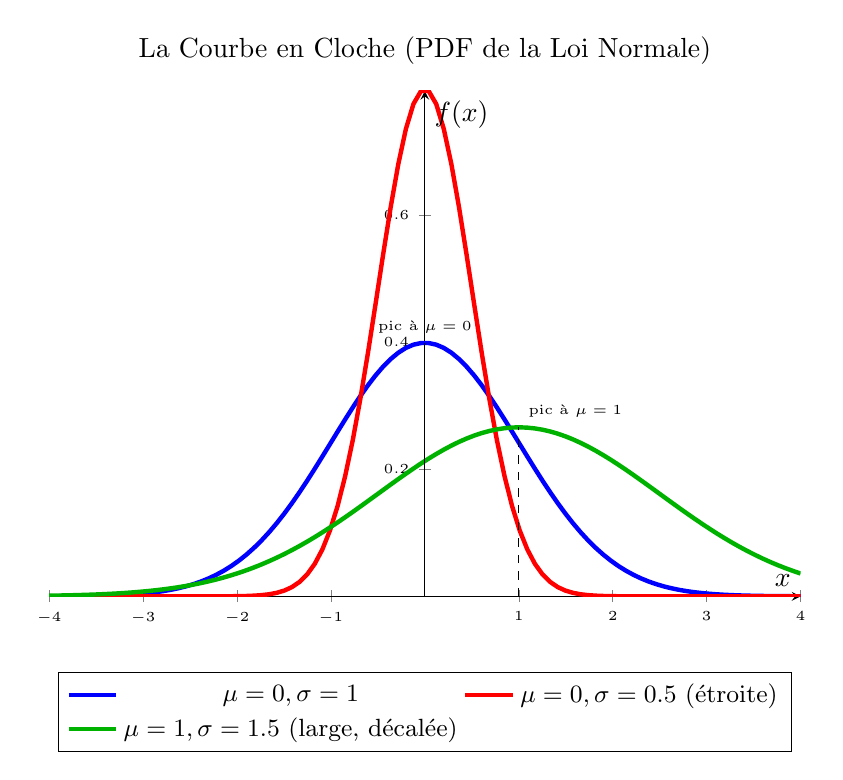
\begin{tikzpicture}
    \begin{axis}[
        title={La Courbe en Cloche (PDF de la Loi Normale)},
        xlabel={$x$},
        ylabel={$f(x)$},
        axis lines=middle,
        no markers,
        samples=100,
        domain=-4:4,
        height=8cm,
        width=\linewidth-1cm,
        tick label style={font=\tiny},
        legend style={at={(0.5,-0.15)}, anchor=north, font=\small},
        legend columns=2
    ]
    % N(0, 1)
    \addplot [blue, ultra thick] {1/(sqrt(2*pi))*exp(-x^2/2)};
    \addlegendentry{$\mu=0, \sigma=1$};
    % N(0, 0.25) => sigma=0.5
    \addplot [red, ultra thick] {1/(0.5*sqrt(2*pi))*exp(-x^2/(2*0.5^2))};
    \addlegendentry{$\mu=0, \sigma=0.5$ (étroite)};
    % N(1, 2.25) => sigma=1.5
    \addplot [green!70!black, ultra thick] {1/(1.5*sqrt(2*pi))*exp(-(x-1)^2/(2*1.5^2))};
    \addlegendentry{$\mu=1, \sigma=1.5$ (large, décalée)};

    \draw [dashed] (axis cs:0,0) -- (axis cs:0, {1/(sqrt(2*pi))}) node[above, font=\tiny] {pic à $\mu=0$}; % Ligne pour mu=0
    \draw [dashed] (axis cs:1,0) -- (axis cs:1, {1/(1.5*sqrt(2*pi))}) node[above right, font=\tiny] {pic à $\mu=1$}; % Ligne pour mu=1
    \end{axis}
\end{tikzpicture}
\par\small\textit{Influence de $\mu$ (position) et $\sigma$ (largeur) sur la forme de la cloche.}
\end{intuitionbox}

\begin{remarquebox}[Pourquoi ce facteur $\frac{1}{\sigma \sqrt{2\pi}}$ ?]
Ce terme devant l'exponentielle peut sembler arbitraire, mais il est absolument essentiel. C'est la \textbf{constante de normalisation}. Son rôle est de s'assurer que l'\textbf{aire totale} sous la courbe de densité vaut exactement 1, ce qui est une condition sine qua non pour toute fonction de densité de probabilité. Sans ce facteur, l'intégrale de $-\infty$ à $+\infty$ ne serait pas égale à 1, et on ne pourrait pas interpréter les aires comme des probabilités. Le $\sigma$ au dénominateur assure également que si la courbe s'élargit (grand $\sigma$), sa hauteur maximale diminue pour conserver une aire constante de 1.
\end{remarquebox}

\subsection{La Loi Normale Centrée Réduite $\mathcal{N}(0, 1)$}

\begin{definitionbox}[Loi Normale Standard (ou Centrée Réduite)]
Un cas particulier extraordinairement utile est la loi normale avec une moyenne $\mu=0$ et une variance $\sigma^2=1$ (donc $\sigma=1$). On l'appelle la \textbf{loi normale standard} ou \textbf{centrée réduite}, et on la note souvent $Z$. Sa PDF est traditionnellement notée $\phi(z)$ :
$$ \phi(z) = \frac{1}{\sqrt{2\pi}} e^{-z^2/2} $$
Sa fonction de répartition (CDF), qui donne $P(Z \le z)$, est notée $\Phi(z)$ :
$$ \Phi(z) = P(Z \le z) = \int_{-\infty}^z \frac{1}{\sqrt{2\pi}} e^{-t^2/2} \, \mathrm{d}t $$
\end{definitionbox}

\begin{intuitionbox}[La Référence Universelle et le Changement d'Unités]
Pourquoi cette loi $\mathcal{N}(0, 1)$ est-elle si centrale ? Imaginez que vous ayez des mesures en degrés Celsius ($\mathcal{N}(\mu_C, \sigma_C^2)$) et d'autres en degrés Fahrenheit ($\mathcal{N}(\mu_F, \sigma_F^2)$). Comment les comparer ? La loi normale standard fournit un \textbf{système d'unités universel}.
\newline
Toute variable normale $X \sim \mathcal{N}(\mu, \sigma^2)$ peut être transformée ("standardisée") en une variable $Z \sim \mathcal{N}(0, 1)$ par un simple changement d'échelle et de position : $Z = (X-\mu)/\sigma$. 
\newline
Cela signifie qu'au lieu de devoir calculer des aires (probabilités) pour une infinité de courbes en cloche différentes (une pour chaque paire $\mu, \sigma$), on peut tout ramener à \textbf{une seule courbe de référence}, $\mathcal{N}(0, 1)$. Les aires sous cette courbe standard ($\Phi(z)$) ont été calculées une fois pour toutes et sont disponibles dans des tables ou des logiciels. On n'a plus qu'à convertir notre problème dans cette "langue" standard, trouver la probabilité, et interpréter le résultat.
\end{intuitionbox}

\begin{remarquebox}[Notation $\phi$ et $\Phi$]
Les symboles $\phi$ (phi minuscule) pour la PDF et $\Phi$ (phi majuscule) pour la CDF de la loi normale standard sont quasi universels. Il est important de ne pas les confondre. $\phi(z)$ est la \textit{hauteur} de la courbe en $z$, tandis que $\Phi(z)$ est l'\textit{aire} sous la courbe à gauche de $z$.
\end{remarquebox}

\begin{remarquebox}[Absence de Primitive Simple]
L'intégrale $\int e^{-t^2/2} \, \mathrm{d}t$, nécessaire pour calculer $\Phi(z)$, n'a \textbf{pas d'expression analytique} en termes de fonctions élémentaires (polynômes, exponentielles, log, sin, cos...). C'est une fonction spéciale, connue sous le nom de \textbf{fonction d'erreur} (liée à $\Phi$ par une transformation simple). C'est la raison pour laquelle on dépend de tables ou de calculs numériques pour obtenir les valeurs de $\Phi(z)$. Heureusement, ces outils sont omniprésents aujourd'hui.
\end{remarquebox}

\subsection{Standardisation : Le Score Z}

\begin{theorembox}[Standardisation d'une Variable Normale]
Si $X \sim \mathcal{N}(\mu, \sigma^2)$, alors la variable $Z$ définie par :
$$ Z = \frac{X - \mu}{\sigma} $$
suit la loi normale standard, $Z \sim \mathcal{N}(0, 1)$.
\end{theorembox}

\begin{intuitionbox}[Mesurer en "Unités d'Écart-Type"]
Transformer $X$ en $Z$ s'appelle \textbf{standardiser} la variable. Le résultat, $z = \frac{x-\mu}{\sigma}$, est appelé le \textbf{Score Z} (ou cote Z). Ce score Z est une mesure \textit{sans unité} qui indique \textbf{à combien d'écarts-types} une valeur observée $x$ se situe par rapport à la moyenne $\mu$ de sa distribution.
\begin{itemize}
    \item $z = 0$ : $x$ est exactement à la moyenne ($\mathbf{x = \mu}$).
    \item $z = +1$ : $x$ est un écart-type \textit{au-dessus} de la moyenne ($\mathbf{x = \mu + \sigma}$).
    \item $z = -2$ : $x$ est deux écarts-types \textit{en dessous} de la moyenne ($\mathbf{x = \mu - 2\sigma}$).
\end{itemize}
Cette transformation est extrêmement utile pour :
\begin{enumerate}
    \item \textbf{Comparer des valeurs} issues de distributions normales différentes. Un score Z de +1.5 a toujours la même signification relative, que l'on parle de QI, de taille, ou de température.
    \item \textbf{Calculer des probabilités} en utilisant la table unique de la loi $\mathcal{N}(0, 1)$.
\end{enumerate}
\end{intuitionbox}

\begin{examplebox}[Comparaison de Performances]
Un étudiant A obtient 80 points à un examen où la moyenne est $\mu_A=70$ et l'écart-type $\sigma_A=5$. Un étudiant B obtient 85 points à un autre examen où $\mu_B=75$ et $\sigma_B=10$. Qui a le mieux réussi relativement à son groupe ?
\newline
Calculons les Z-scores :
$$ Z_A = \frac{80 - 70}{5} = \frac{10}{5} = +2.0 $$
$$ Z_B = \frac{85 - 75}{10} = \frac{10}{10} = +1.0 $$
L'étudiant A a un score Z plus élevé (+2.0 contre +1.0), ce qui signifie qu'il se situe plus d'écarts-types au-dessus de la moyenne de son groupe que l'étudiant B. L'étudiant A a donc relativement mieux réussi.
\end{examplebox}

\subsection{Propriétés Importantes de la Loi Normale}

\begin{theorembox}[Stabilité par Transformation Linéaire]
Si $X \sim \mathcal{N}(\mu, \sigma^2)$ et $Y = aX + b$ (avec $a \neq 0$), alors $Y$ suit aussi une loi normale :
$$ Y \sim \mathcal{N}(a\mu + b, \, (a\sigma)^2) $$
L'espérance est transformée linéairement ($E[aX+b] = aE[X]+b$), et la variance est multipliée par $a^2$ ($\text{Var}(aX+b) = a^2\text{Var}(X)$).
\end{theorembox}

\begin{examplebox}[Changement d'Unités]
Si la température en Celsius $T_C$ suit $\mathcal{N}(20, 5^2)$, quelle est la loi de la température en Fahrenheit $T_F = \frac{9}{5}T_C + 32$ ?
\newline
$a = 9/5$, $b=32$.
\newline
Nouvelle moyenne : $E[T_F] = \frac{9}{5}(20) + 32 = 36 + 32 = 68$.
\newline
Nouvel écart-type : $\sigma_{T_F} = |a|\sigma_{T_C} = \frac{9}{5}(5) = 9$. Nouvelle variance : $\sigma_{T_F}^2 = 9^2 = 81$.
\newline
Donc, $T_F \sim \mathcal{N}(68, 9^2)$.
\end{examplebox}

\begin{theorembox}[Stabilité par Addition (Indépendance)]
Si $X \sim \mathcal{N}(\mu_X, \sigma_X^2)$ et $Y \sim \mathcal{N}(\mu_Y, \sigma_Y^2)$ sont des variables aléatoires \textbf{indépendantes}, alors leur somme $S = X + Y$ suit aussi une loi normale :
$$ S \sim \mathcal{N}(\mu_X + \mu_Y, \, \sigma_X^2 + \sigma_Y^2) $$
Les moyennes s'ajoutent, et (grâce à l'indépendance) les variances s'ajoutent.
\end{theorembox}

\begin{remarquebox}[Attention à l'Indépendance]
La propriété d'addition des variances ($\sigma_S^2 = \sigma_X^2 + \sigma_Y^2$) est cruciale et ne tient \textbf{que si $X$ et $Y$ sont indépendantes}. Si elles ne le sont pas, la variance de la somme inclut un terme de covariance : $\text{Var}(X+Y) = \text{Var}(X) + \text{Var}(Y) + 2\text{Cov}(X, Y)$. Cependant, la somme de variables normales (même dépendantes) reste normale (si elles sont conjointement normales).
\end{remarquebox}

\begin{examplebox}[Poids Total]
Le poids d'une pomme suit $\mathcal{N}(150g, 10^2)$. Le poids d'une orange suit $\mathcal{N}(200g, 15^2)$. On suppose les poids indépendants. Quel est la loi du poids total d'une pomme et d'une orange ?
\newline
Soit $P$ le poids de la pomme, $O$ celui de l'orange. $T = P+O$.
\newline
$E[T] = E[P] + E[O] = 150 + 200 = 350g$.
\newline
$\text{Var}(T) = \text{Var}(P) + \text{Var}(O) = 10^2 + 15^2 = 100 + 225 = 325$.
\newline
Donc, $T \sim \mathcal{N}(350, 325)$. L'écart-type du poids total est $\sqrt{325} \approx 18.03g$.
\end{examplebox}

\subsection{La Règle Empirique (68-95-99.7)}

\begin{theorembox}[Règle Empirique]
Pour toute variable $X \sim \mathcal{N}(\mu, \sigma^2)$ :
\begin{itemize}
    \item $P(\mu - \sigma \le X \le \mu + \sigma) \approx 0.6827$ (Environ \textbf{68\%} des valeurs dans $\mu \pm \sigma$).
    \item $P(\mu - 2\sigma \le X \le \mu + 2\sigma) \approx 0.9545$ (Environ \textbf{95\%} des valeurs dans $\mu \pm 2\sigma$).
    \item $P(\mu - 3\sigma \le X \le \mu + 3\sigma) \approx 0.9973$ (Environ \textbf{99.7\%} des valeurs dans $\mu \pm 3\sigma$).
\end{itemize}
\end{theorembox}

\begin{intuitionbox}[Repères Essentiels sur la Cloche]
Cette règle, dérivée directement des aires sous la courbe $\mathcal{N}(0, 1)$ entre $z=\pm 1$, $z=\pm 2$ et $z=\pm 3$, fournit des repères extrêmement utiles pour interpréter l'écart-type $\sigma$. Elle nous dit où se trouve la grande majorité des données.
\newline
Une observation qui tombe en dehors de l'intervalle $\mu \pm 3\sigma$ est très inhabituelle (elle n'a que 0.3pct de chances de se produire). C'est souvent considéré comme une \textit{valeur aberrante} (outlier) potentielle.
\end{intuitionbox}

\subsection{Calcul de Probabilités Normales}

\begin{examplebox}[Utilisation du Z-score]
Supposons que le QI d'une population suit $\mathcal{N}(100, 15^2)$. Quelle est la probabilité $P(X > 130)$ ?

1.  \textbf{Standardiser :} $z = \frac{130 - 100}{15} = 2$. On cherche $P(Z > 2)$.
2.  \textbf{Utiliser la CDF Standard :} $P(Z > 2) = 1 - P(Z \le 2) = 1 - \Phi(2)$.
3.  \textbf{Chercher dans la table / Calculer :} $\Phi(2) \approx 0.9772$.
4.  \textbf{Résultat :} $P(X > 130) = 1 - 0.9772 = 0.0228$.
\end{examplebox}

\begin{examplebox}[Probabilité entre deux valeurs]
Quelle est la probabilité $P(85 \le X \le 115)$ ?

1.  \textbf{Standardiser :} $z_1 = \frac{85 - 100}{15} = -1$, $z_2 = \frac{115 - 100}{15} = 1$. On cherche $P(-1 \le Z \le 1)$.
2.  \textbf{Utiliser la CDF Standard :} $P(-1 \le Z \le 1) = \Phi(1) - \Phi(-1)$.
3.  \textbf{Utiliser la symétrie :} $\Phi(-z) = 1 - \Phi(z)$. Donc $\Phi(-1) = 1 - \Phi(1)$.
    $P(-1 \le Z \le 1) = \Phi(1) - (1 - \Phi(1)) = 2\Phi(1) - 1$.
4.  \textbf{Chercher dans la table / Calculer :} $\Phi(1) \approx 0.8413$.
5.  \textbf{Résultat :} $P(85 \le X \le 115) \approx 2(0.8413) - 1 = 1.6826 - 1 = 0.6826$.
\end{examplebox}

\begin{examplebox}[Trouver une valeur pour une probabilité donnée (Problème Inverse)]
Quel est le QI minimum requis pour être dans le top 10\% de la population ? ($\mu=100, \sigma=15$).

1.  \textbf{Trouver le Z-score correspondant :} On cherche $x$ tel que $P(X > x) = 0.10$. Cela équivaut à $P(Z > z) = 0.10$, où $z = (x-100)/15$.
    Si $P(Z > z) = 0.10$, alors $P(Z \le z) = \Phi(z) = 1 - 0.10 = 0.90$.
2.  \textbf{Chercher dans la table inverse / Calculer :} On cherche la valeur $z$ pour laquelle l'aire à gauche est 0.90. On trouve $z \approx 1.28$.
3.  \textbf{Convertir en X :} On utilise la relation $z = (x-\mu)/\sigma$ pour trouver $x$:
    $1.28 = \frac{x - 100}{15}$
    $x = 100 + 1.28 \times 15 = 100 + 19.2 = 119.2$.
    Il faut un QI d'environ 119.2 pour être dans le top 10\%.
\end{examplebox}

\subsection{Le Théorème Central Limite (TCL)}

\begin{theorembox}[Théorème Central Limite (TCL)]
Soit $X_1, X_2, \dots, X_n$ une suite de variables aléatoires indépendantes et identiquement distribuées (i.i.d.) avec une espérance $\mu$ et une variance $\sigma^2$ finies. Alors, la distribution de la \textbf{moyenne empirique} $\bar{X}_n = \frac{1}{n}\sum_{i=1}^n X_i$ converge vers une loi normale lorsque $n$ tend vers l'infini. Plus précisément :
$$ \frac{\bar{X}_n - \mu}{\sigma/\sqrt{n}} \xrightarrow{d} \mathcal{N}(0, 1) \quad \text{quand } n \to \infty $$
Cela signifie que pour $n$ grand, $\bar{X}_n$ suit approximativement la loi $\mathcal{N}\left(\mu, \frac{\sigma^2}{n}\right)$.
\end{theorembox}

\begin{intuitionbox}[La Convergence Universelle vers la Cloche ]
Le TCL est l'un des joyaux des probabilités. Il nous dit quelque chose de remarquable : \textbf{peu importe la forme de la distribution initiale} des $X_i$ (elle peut être quelconque : uniforme, exponentielle, bimodale, inconnue...), la \textbf{moyenne d'un grand nombre d'observations indépendantes issues de cette distribution tendra inévitablement à suivre une distribution normale} ! 
\newline
Pourquoi ? Intuitivement, quand on fait la moyenne de nombreuses variables aléatoires, les extrêmes ont tendance à se compenser. Une valeur très grande sera souvent moyennée avec une valeur très petite, et le résultat se rapprochera de la moyenne générale $\mu$. Les fluctuations autour de $\mu$ résultent de la combinaison de nombreux petits écarts aléatoires, et cette combinaison tend à produire la forme symétrique de la cloche gaussienne.
\newline
C'est la raison fondamentale de l'omniprésence de la loi normale :
\begin{itemize}
    \item \textbf{Phénomènes Naturels :} Beaucoup de caractéristiques biologiques (taille, poids...) résultent de l'influence combinée de nombreux gènes et facteurs environnementaux.
    \item \textbf{Erreurs de Mesure :} Les erreurs dans les mesures physiques sont souvent la somme de multiples petites perturbations aléatoires.
    \item \textbf{Processus Industriels :} La qualité d'un produit peut dépendre de la moyenne de nombreuses variables de production.
    \item \textbf{Finance :} Les rendements boursiers sur une période peuvent être vus comme la somme de petits changements journaliers.
\end{itemize}
Le TCL nous assure que même si les composantes individuelles ne sont pas normales, leur somme ou leur moyenne le deviendra approximativement si elles sont assez nombreuses et indépendantes.
\end{intuitionbox}

\begin{remarquebox}[Conditions d'Application et Approximations]
Le TCL est un théorème \textit{limite} ($n \to \infty$), mais l'approximation normale pour $\bar{X}_n$ est souvent jugée acceptable en pratique dès que $n$ est "suffisamment grand". La règle empirique la plus courante est $n \ge 30$, mais ce seuil dépend fortement de l'asymétrie de la distribution initiale. Si la distribution de départ est déjà proche d'une cloche, l'approximation sera bonne même pour des $n$ plus petits. Si elle est très asymétrique (comme une exponentielle), il faudra un $n$ plus grand.
\newline
Le TCL justifie aussi les approximations suivantes :
\begin{itemize}
    \item \textbf{Binomiale $\rightarrow$ Normale :} Si $X \sim \text{Bin}(n, p)$ avec $np \ge 5$ et $n(1-p) \ge 5$, alors $X \approx \mathcal{N}(np, np(1-p))$. C'est logique car une binomiale est une somme de $n$ Bernoulli i.i.d.
    \item \textbf{Poisson $\rightarrow$ Normale :} Si $Y \sim \text{Poisson}(\lambda)$ avec $\lambda$ grand (par ex. $\lambda \ge 20$), alors $Y \approx \mathcal{N}(\lambda, \lambda)$.
\end{itemize}
\textbf{Correction de Continuité :} Lors de l'approximation d'une variable discrète (Binomiale, Poisson) par une variable continue (Normale), on améliore souvent la précision en ajustant les bornes de l'intervalle. Par exemple, pour calculer $P(X \le k)$ où $X$ est discrète, on calcule $P(Y \le k+0.5)$ où $Y$ est l'approximation normale. Pour $P(X=k)$, on calcule $P(k-0.5 \le Y \le k+0.5)$.
\end{remarquebox}